% \begin{figure}[t]
% \minipage{0.33\textwidth}
%   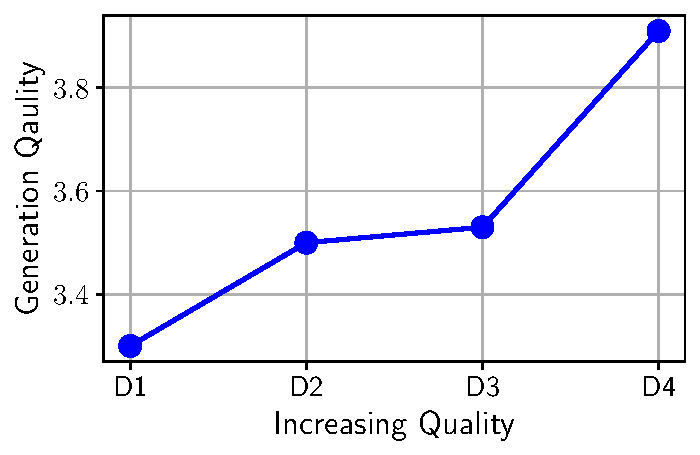
\includegraphics[width=\linewidth]{figs/quality.pdf}
%   \caption{(a) Quality}\label{fig:quality}
% \endminipage\hfill
% \minipage{0.33\textwidth}
%   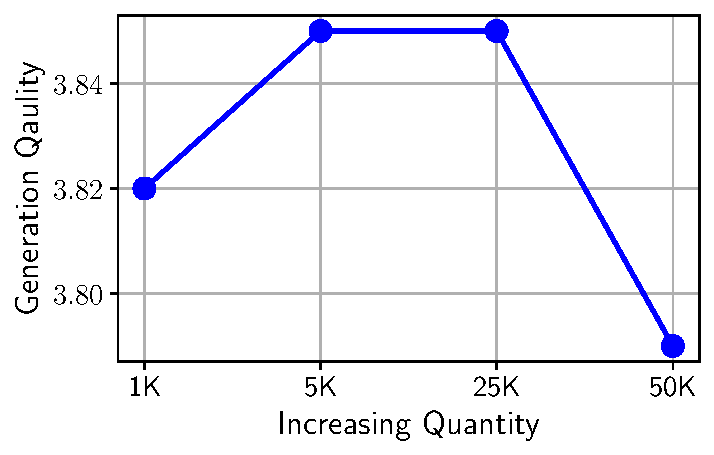
\includegraphics[width=\linewidth]{figs/quantity.pdf}
%   \caption{(b) Quantity}\label{fig:quantity}
% \endminipage\hfill
% \minipage{0.33\textwidth}%
%   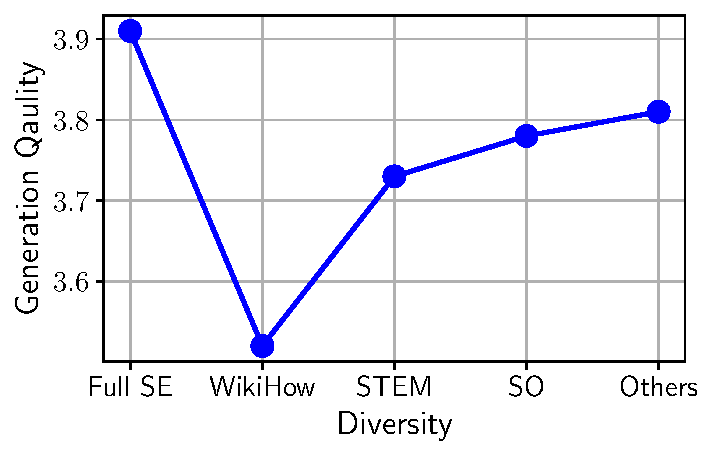
\includegraphics[width=\linewidth]{figs/diversity.pdf}
%  \caption{(c) Diversity}\label{fig:diversity}
% \endminipage
%   \caption{Ablations on the effects of supervised fine-tuning data w.r.t. quality, quantity and diversity.
% \label{fig:abl}}
% \end{figure}


\begin{figure}
     \centering
     \begin{subfigure}[b]{0.323\textwidth}
         \centering
         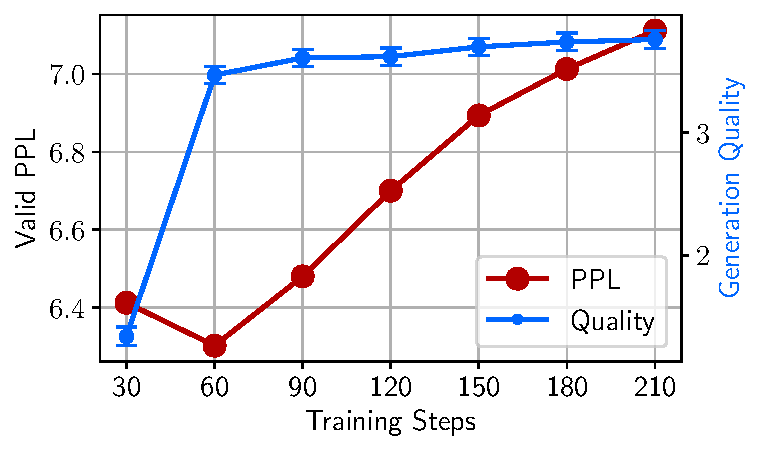
\includegraphics[width=\linewidth]{figs/ppl_7b.pdf}
         \caption{LIMA 7B}
         \label{fig:ppl:7b}
     \end{subfigure}
     \hfill
     \begin{subfigure}[b]{0.323\textwidth}
         \centering
         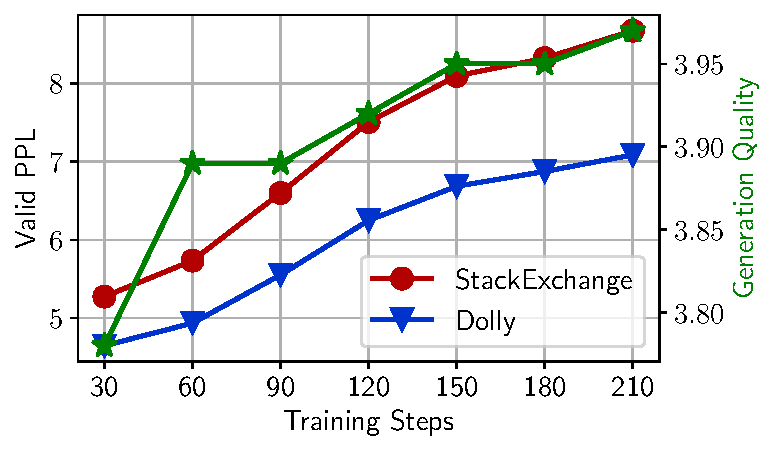
\includegraphics[width=\linewidth]{figs/ppl_30b.pdf}
         \caption{LIMA 30B}
         \label{fig:ppl:30b}
     \end{subfigure}
     \hfill
     \begin{subfigure}[b]{0.323\textwidth}
         \centering
         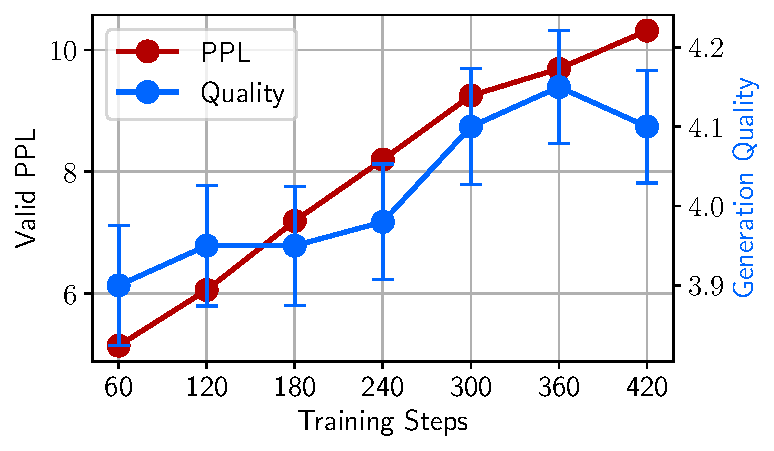
\includegraphics[width=\linewidth]{figs/ppl_65b.pdf}
         \caption{LIMA 65B}
         \label{fig:ppl:65B}
     \end{subfigure}
        \caption{Validation PPL and generation quality evaluated by ChatGPT.}
        \label{fig:ppl}
\end{figure}


\begin{figure}
     \centering
     \begin{subfigure}[b]{0.45\textwidth}
         \centering
         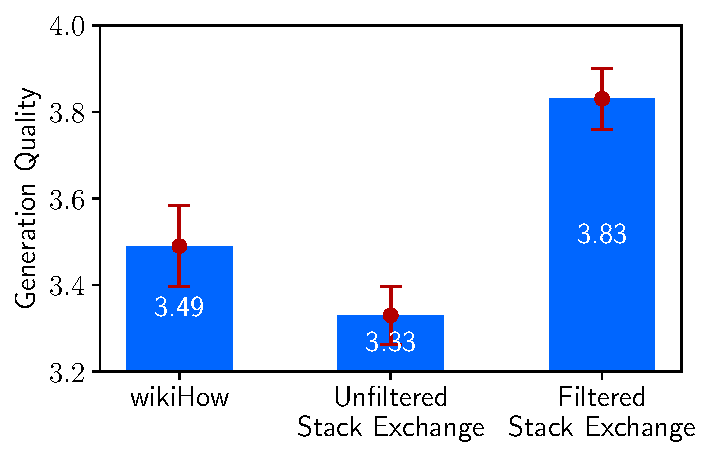
\includegraphics[width=\linewidth]{figs/quality_bar.pdf}
         \caption{Different training data. \omer{add error bars / confidence interval / boxplot}}
         \label{fig:quality}
     \end{subfigure}
     \hfill
     \begin{subfigure}[b]{0.45\textwidth}
         \centering
         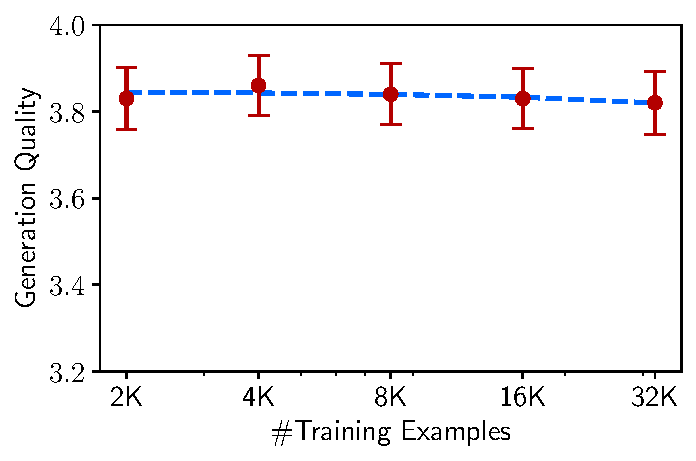
\includegraphics[width=\linewidth]{figs/quantity_se.pdf}
         \caption{Varying training data size on SE. \omer{here too}}
         \label{fig:ppl:65B}
     \end{subfigure}
        \caption{Ablation studies.}
        \label{fig:abl}
\end{figure}

% \pfliu{
%         (1) Figure (a): Does generation quality refer to the likert score (1-6) in automatic evaluation in y-axis, and what do D1, D2, D3 and D4 in represent?  (2) Figure (b) : How are quality and diversity controlled as quantity increases
%         (3) Figure (c) : Similarly, is the x-axis means that the effect 
%  of one specific domain (e.g., Full SE)? Similarly, how are the,quality and quantity quantities controlled in this situation
%  (4) add which model (7B or 30B) is used. (5) we potentially could break down the overall generation quality in terms of different scenarios (e.g., writing, math, code etc)}